%! TeX root = ../main.tex
\chapter{METODOLOGI}
\label{chap:metodologipenelitian}

\section{Diagram Alir Penelitian}
\label{sec:diagramalir}

Metodologi penelitian ini dilakukan melalui tahapan sebagaimana ditunjukkan pada Gambar~\ref{fig:alir-metodologi}. Penelitian dimulai dengan studi literatur dan identifikasi kebutuhan serta batasan sistem, kemudian dilanjutkan dengan perancangan sistem dan prototipe serta penyusunan dataset sintetis yang melalui proses \emph{quality control} sebelum dilakukan pembagian dataset. Setelah itu, proses \emph{fine-tuning} Qwen3-1.7B dan persiapan lingkungan \emph{deployment} pada Raspberry Pi 5 4GB dilakukan sebagai tahap persiapan menuju implementasi pemrosesan dan integrasi sistem. Sistem yang telah diimplementasikan kemudian melalui tahap \emph{pilot} dan pemilihan konfigurasi sebelum konfigurasi serta protokol pengujian ditetapkan. Tahap selanjutnya adalah pengujian sistem, analisis hasil pengujian, dan penarikan kesimpulan.

\begin{figure}[H]
  \centering
  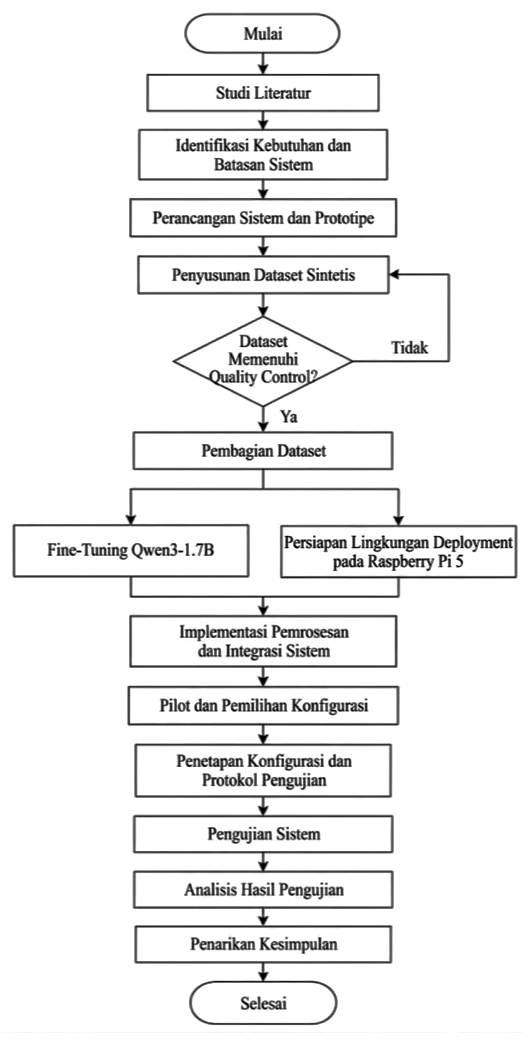
\includegraphics[height=13.5cm]{gambar/gambar-3-1.png}
  \caption{Diagram Alir Metodologi Penelitian}
  \label{fig:alir-metodologi}
\end{figure}

\section{Studi Literatur}
\label{sec:studiliteratur}

Studi literatur dilakukan untuk memperoleh dasar dalam perancangan dan pengujian sistem \emph{Edge AI} yang dikembangkan. Literatur yang dikaji mencakup dokumentasi klinis berbasis SOAP, \emph{Speech-to-Text}, penggunaan \emph{Small Language Model} untuk pemrosesan teks klinis, \emph{Edge AI}, \emph{quantization}, serta metode evaluasi kualitas keluaran dan performa \emph{deployment}.

Hasil studi literatur digunakan sebagai dasar dalam menentukan pendekatan pemrosesan, pemilihan model, penyusunan metode evaluasi, serta parameter yang diperlukan pada tahap implementasi dan pengujian. Pembahasan pada bagian ini difokuskan pada penggunaan literatur sebagai dasar metodologi, sedangkan teori dan penelitian terdahulu dibahas pada Bab II.

\section{Gambaran Umum Sistem Penelitian}
\label{sec:gambaranumum}

Penelitian ini mengembangkan sistem \emph{Edge AI} yang ditujukan untuk membantu menghasilkan \emph{draft} dokumentasi SOAP berdasarkan percakapan dokter--pasien. Sistem dirancang dalam bentuk perangkat mandiri dengan Raspberry Pi 5 4GB sebagai perangkat komputasi utama. Pemrosesan AI utama dilakukan secara lokal atau \emph{on-device} sehingga proses pengolahan percakapan hingga pembentukan \emph{draft} SOAP tidak bergantung pada layanan komputasi \emph{cloud} sebagai bagian dari alur utama sistem.

Masukan sistem berupa audio percakapan dokter--pasien yang diproses menjadi transkrip menggunakan \emph{Speech-to-Text} (STT). Transkrip tersebut kemudian diproses melalui \emph{pipeline} berbasis \emph{Small Language Model} (SLM) yang mencakup ekstraksi informasi klinis, \emph{Context Harness}, generasi SOAP, serta validasi berbasis aturan. Hubungan antarblok proses dan perubahan data pada setiap tahap ditunjukkan pada Gambar~\ref{fig:blok-sistem} pada Subbab~\ref{subsec:arsitektursistem}.

\emph{Draft} SOAP yang dihasilkan selanjutnya diteruskan ke lingkungan EMR/SIMRS untuk ditinjau dan diedit oleh dokter. Sistem tidak ditujukan sebagai \emph{Clinical Decision Support System} maupun sistem diagnosis otomatis, sehingga keluaran sistem tetap berupa \emph{draft} dokumentasi dan keputusan akhir terhadap isi rekam medis berada pada dokter. Evaluasi penelitian difokuskan pada tingkat \emph{groundedness draft} SOAP terhadap informasi dalam \emph{encounter} serta kelayakan \emph{deployment} sistem secara \emph{on-device} pada Raspberry Pi 5 4GB.

\section{Perancangan Sistem dan Prototipe}
\label{sec:perancangansistem}

\subsection{Arsitektur Sistem}
\label{subsec:arsitektursistem}

Sistem \emph{Edge AI} dirancang untuk mengolah percakapan dokter--pasien menjadi \emph{draft} SOAP dengan pemrosesan AI utama dilakukan secara lokal pada Raspberry Pi. Alur sistem terdiri atas akuisisi audio, \emph{Speech-to-Text} (STT), pemrosesan pembicara yang bersifat opsional, ekstraksi informasi klinis, \emph{Context Harness}, generasi SOAP, validasi berbasis aturan, serta integrasi menuju EMR/SIMRS. Hubungan antarblok proses dan perubahan data pada setiap tahap ditunjukkan pada Gambar~\ref{fig:blok-sistem}.

\begin{figure}[H]
  \centering
  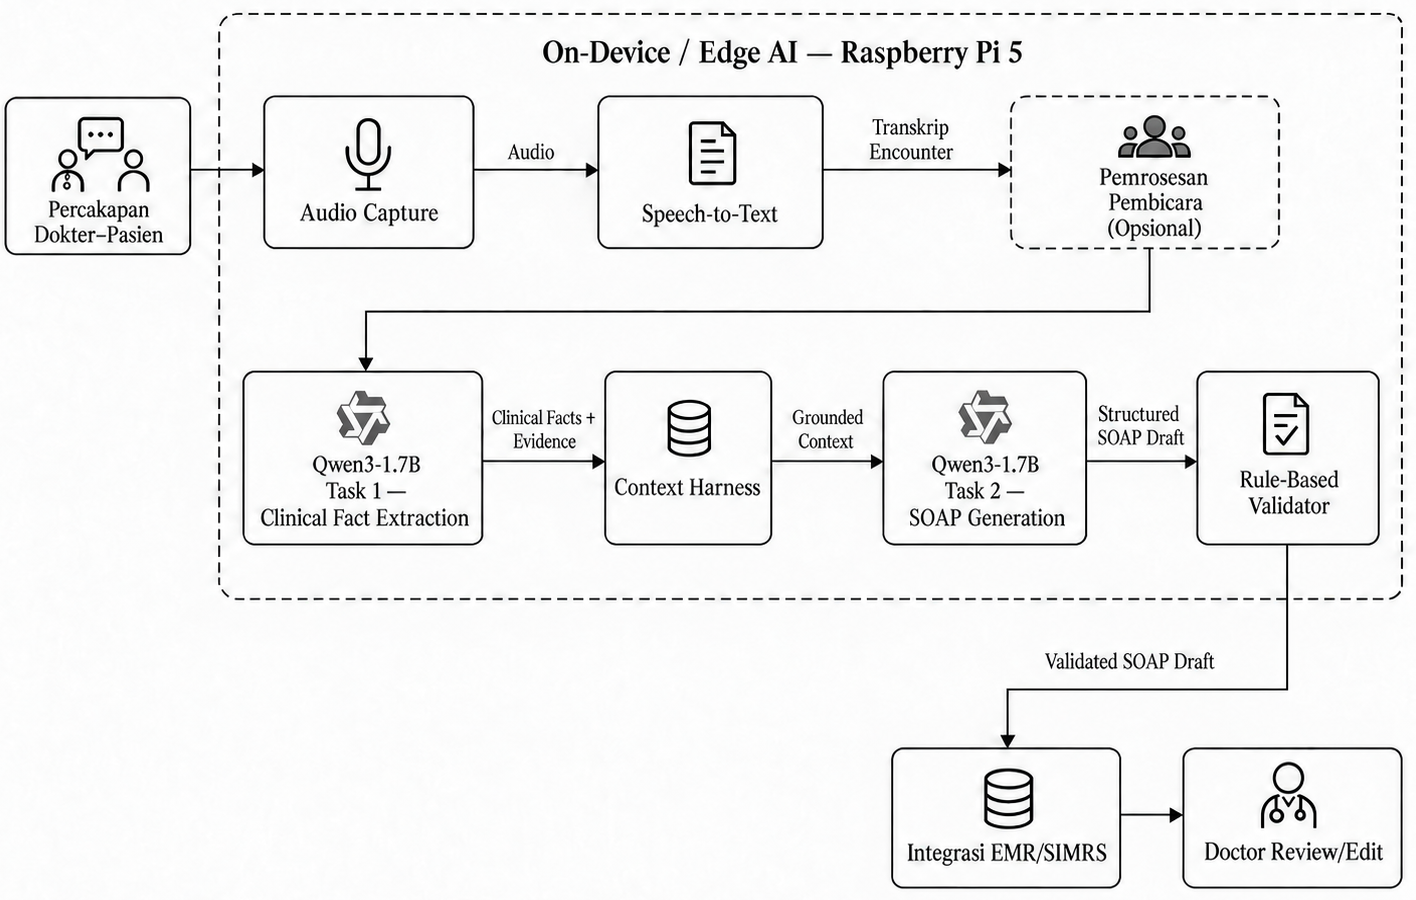
\includegraphics[width=\textwidth]{gambar/gambar-3-2.png}
  \caption{Diagram Blok Kerja Sistem Edge AI}
  \label{fig:blok-sistem}
\end{figure}

Pemrosesan berbasis \emph{Small Language Model} menggunakan satu model Qwen3-1.7B secara berurutan untuk dua tugas yang berbeda. Tahap pertama digunakan untuk mengekstraksi informasi klinis beserta \emph{evidence} dari transkrip \emph{encounter}, sedangkan tahap kedua digunakan untuk menghasilkan \emph{draft} SOAP berdasarkan konteks yang telah disusun oleh \emph{Context Harness}. \emph{Draft} yang dihasilkan kemudian diperiksa oleh \emph{rule-based validator} dan diteruskan melalui lapisan integrasi menuju EMR/SIMRS untuk ditinjau dan diedit oleh dokter.

\subsection{Perancangan Perangkat Keras}
\label{subsec:perangkatkeras}

Perangkat \emph{Edge AI} dirancang menggunakan Raspberry Pi 5 4GB sebagai unit komputasi utama dengan media penyimpanan microSD 64GB dan sistem pendinginan aktif. Perangkat dilengkapi mikrofon USB untuk akuisisi percakapan, tombol tekan (\emph{push button}) untuk mengontrol proses perekaman, LED status sebagai indikator kondisi perangkat, serta catu daya USB-C 5V/5A 27W. Seluruh komponen direncanakan ditempatkan dalam sebuah wadah pelindung (\emph{enclosure}) sehingga dapat digunakan sebagai perangkat mandiri pada meja pemeriksaan dokter.

\emph{Enclosure} dirancang dengan mempertimbangkan penempatan komponen, ruang untuk sistem pendinginan, ventilasi, serta akses terhadap konektor, tombol, dan indikator. Bentuk dan dimensi \emph{enclosure} akan disesuaikan dengan komponen fisik yang digunakan dan tidak diperlakukan sebagai variabel utama penelitian.

Kecukupan Raspberry Pi 5 4GB dari sisi penggunaan memori, waktu pemrosesan, dan kondisi termal tidak diasumsikan pada tahap perancangan, melainkan dievaluasi melalui pengujian kelayakan \emph{deployment}.

\subsection{Perancangan Akuisisi dan Pemrosesan Audio}
\label{subsec:akuisisiaudio}

Akuisisi percakapan dilakukan menggunakan mikrofon USB yang terhubung langsung ke Raspberry Pi. Audio hasil perekaman disiapkan dalam format yang konsisten sebagai masukan untuk proses \emph{Speech-to-Text}, yaitu audio mono dengan \emph{sample rate} 16 kHz dan format PCM 16-bit dalam berkas WAV. Apabila mikrofon menghasilkan format audio yang berbeda, dilakukan normalisasi sebelum audio diteruskan ke modul STT.

Pemrosesan audio pada penelitian ini dibatasi pada normalisasi yang diperlukan untuk memperoleh masukan STT yang konsisten. Pemrosesan tambahan seperti \emph{noise suppression}, \emph{beamforming}, atau \emph{speech enhancement} tidak digunakan sebagai \emph{baseline} agar tidak menambah kompleksitas dan variabel penelitian yang tidak berkaitan langsung dengan tujuan utama sistem.

Pemilihan mikrofon, penguatan (\emph{gain}), posisi pemasangan, dan konfigurasi penggunaannya akan dikonfirmasi melalui tahap rintisan (\emph{pilot}) sehingga kualitas akuisisi audio tidak diasumsikan sebelum dilakukan pengujian.

\subsection{Perancangan Pipeline AI Berbasis SLM}
\label{subsec:pipelineai}

\emph{Pipeline} AI dirancang menggunakan satu model Qwen3-1.7B yang dijalankan secara berurutan untuk dua tugas. Tahap pertama digunakan untuk mengekstraksi fakta klinis beserta \emph{evidence} dari transkrip percakapan. Hasil tersebut kemudian diproses oleh \emph{Context Harness} untuk menyiapkan konteks sebelum digunakan pada tahap kedua dalam menghasilkan \emph{draft} SOAP.

Informasi yang diteruskan antar-tahap tetap mempertahankan keterkaitannya dengan bagian percakapan yang menjadi sumbernya. \emph{Pipeline} ini tidak menggunakan model bahasa tambahan maupun mekanisme pengambilan pengetahuan klinis eksternal. \emph{Draft} SOAP yang terbentuk selanjutnya diteruskan ke validator berbasis aturan sebelum masuk ke tahap integrasi.

\subsection{Perancangan Validator dan Integrasi EMR/SIMRS}
\label{subsec:perancanganvalidator}

Validator dirancang sebagai komponen programatik untuk memeriksa keluaran SOAP sebelum diteruskan ke lingkungan EMR/SIMRS. Setelah melalui proses validasi, \emph{draft} SOAP diubah secara deterministik menjadi format yang dapat digunakan pada tahap integrasi tanpa melakukan inferensi atau menambahkan informasi klinis baru.

Komunikasi antara perangkat \emph{Edge AI} dan peramban (\emph{browser}) dirancang menggunakan \emph{Integration Interface} melalui komunikasi HTTP pada jaringan lokal dengan mekanisme \emph{polling}. Pada sisi peramban digunakan \emph{Chrome Extension Manifest V3} yang berfungsi sebagai penghubung antara perangkat dan halaman EMR/SIMRS.

Pemetaan kolom (\emph{field}) dibuat dapat dikonfigurasi sehingga mekanisme integrasi dapat digunakan pada tampilan dengan kolom SOAP terpisah maupun satu kolom catatan klinis. Mekanisme integrasi juga mempertahankan identitas \emph{encounter} dan \emph{payload} untuk mengurangi risiko \emph{draft} masuk ke \emph{encounter} yang salah atau diproses secara berulang.

\section{Persiapan Data dan Model}
\label{sec:persiapandata}

\subsection{Penyusunan Dataset Sintetis dan Ground Truth}
\label{subsec:datasetsintetis}

Dataset penelitian direncanakan menggunakan percakapan klinis sintetis yang disusun dalam bentuk \emph{encounter} dokter--pasien. Setiap \emph{encounter} memiliki transkrip referensi yang digunakan sebagai dasar untuk menyusun fakta klinis, \emph{evidence}, dan referensi SOAP. \emph{Ground truth} tidak dibuat dari hasil STT agar kesalahan transkripsi dapat dipisahkan dari kesalahan pemrosesan klinis pada tahap evaluasi.

Fakta klinis yang telah diverifikasi kemudian ditandai berdasarkan kebutuhan representasinya pada SOAP, yaitu informasi yang harus tercakup, informasi yang bersifat opsional, atau informasi yang tidak menjadi target dokumentasi. Dataset sintetis selanjutnya melalui pemeriksaan dan koreksi klinis sebelum digunakan sebagai \emph{ground truth} penelitian.

\subsection{Anotasi dan Quality Control Dataset}
\label{subsec:annotationqc}

Proses anotasi dilakukan dengan mengidentifikasi informasi klinis pada transkrip, menghubungkannya dengan \emph{evidence} yang sesuai, menyatukan informasi yang memiliki makna sama, serta menyusun referensi SOAP berdasarkan aturan klinis yang telah ditetapkan.

Setelah anotasi selesai, dilakukan kendali mutu (\emph{quality control}) untuk memastikan konsistensi antara transkrip, fakta klinis, \emph{evidence}, dan referensi SOAP. Data yang belum sesuai diperbaiki, sedangkan kasus yang masih memiliki perbedaan interpretasi diselesaikan melalui proses adjudikasi sebelum diterima sebagai \emph{ground truth}. Konfigurasi operasional peninjau klinis (\emph{clinical reviewer}) akan ditetapkan sebelum produksi dataset final.

\subsection{Pembagian Dataset dan Pencegahan Data Leakage}
\label{subsec:dataleakage}

Dataset direncanakan dibagi untuk kebutuhan pelatihan, pemilihan konfigurasi, dan pengujian akhir. Pembagian dilakukan dengan memperhatikan keterkaitan antar-skenario sehingga data yang berasal dari skenario, parafrasa, atau variasi audio yang sama tidak tersebar secara tidak terkendali pada kelompok yang berbeda.

Data pengujian akhir tidak digunakan dalam proses pelatihan maupun pemilihan konfigurasi. Mekanisme pengelompokan, proporsi pembagian, dan prosedur pemeriksaan kebocoran data (\emph{data leakage}) ditetapkan sebelum produksi dataset dan pelaksanaan eksperimen final.

\subsection{Fine-Tuning SLM}
\label{subsec:finetuningslm}

\emph{Fine-tuning} direncanakan menggunakan pendekatan \emph{Supervised Fine-Tuning} (SFT) dengan LoRA pada laptop atau PC. Proses ini digunakan untuk menyesuaikan Qwen3-1.7B terhadap kebutuhan ekstraksi informasi klinis dan penyusunan SOAP terstruktur.

Model hasil \emph{fine-tuning} kemudian disiapkan untuk \emph{deployment} pada Raspberry Pi. Parameter pelatihan dan peningkatan kualitas yang diperoleh belum dianggap sebagai hasil penelitian sebelum proses \emph{fine-tuning} dan evaluasi dilakukan.

\subsection{Persiapan Konfigurasi Deployment dan Quantization}
\label{subsec:quantization}

Model yang telah dipersiapkan direncanakan dikonversi ke format GGUF dan dijalankan menggunakan \emph{llama.cpp}. Untuk \emph{deployment}, beberapa konfigurasi kuantisasi (\emph{quantization}) disiapkan, yaitu Q8\_0, Q5\_K\_M, dan Q4\_K\_M.

Konfigurasi tersebut dibandingkan pada tahap pemilihan konfigurasi berdasarkan kebutuhan sumber daya, performa pemrosesan, dan kualitas keluaran. Konfigurasi yang digunakan pada pengujian akhir ditentukan setelah proses tersebut dilakukan dan tidak diasumsikan sebelumnya sebagai konfigurasi terbaik.

\section{Implementasi dan Pemrosesan Sistem}
\label{sec:implementasisistem}

\subsection{Audio Capture}
\label{subsec:audiocapture}

Proses pemrosesan sistem dimulai ketika pengguna mengaktifkan perekaman melalui tombol tekan (\emph{push button}) pada perangkat. Sistem kemudian merekam percakapan dokter--pasien menggunakan mikrofon USB sampai proses perekaman dihentikan oleh pengguna.

Setelah perekaman selesai, audio dinormalisasi ke format yang digunakan oleh \emph{pipeline} STT. Audio yang telah siap kemudian diteruskan ke tahap \emph{Speech-to-Text} untuk menghasilkan transkrip \emph{encounter}. Titik ketika audio selesai disiapkan juga digunakan sebagai awal pengukuran waktu pemrosesan setelah perekaman pada evaluasi \emph{deployment}.

\subsection{Speech-to-Text}
\label{subsec:speechtotext}

Tahap \emph{Speech-to-Text} digunakan untuk mengubah audio percakapan menjadi transkrip yang selanjutnya digunakan oleh \emph{pipeline} pemrosesan klinis. STT direncanakan menggunakan Whisper Small \emph{multilingual} yang dijalankan secara lokal melalui \texttt{whisper.cpp}.

Hasil STT disusun menjadi representasi transkrip yang mempertahankan urutan percakapan dan informasi waktu yang diperlukan oleh tahap berikutnya. Kualitas hasil transkripsi kemudian dievaluasi secara terpisah untuk membantu menganalisis pengaruh kesalahan STT terhadap keluaran akhir sistem.

\subsection{Optional Speaker Processing}
\label{subsec:speakerprocessing}

Setelah proses STT, sistem dapat menggunakan tahap pemrosesan penutur (\emph{speaker processing}) untuk membantu membedakan sumber informasi dalam percakapan. Tahap ini bersifat opsional dan tidak menjadi syarat agar transkrip dapat diteruskan ke proses ekstraksi informasi klinis.

Diarisasi (\emph{diarization}) dapat digunakan untuk membantu menentukan siapa yang berbicara pada bagian tertentu dari percakapan. Namun, diarisasi tidak secara otomatis menentukan peran pembicara. Penggunaan tahap ini pada konfigurasi akhir ditentukan berdasarkan hasil pengujian terhadap manfaat \emph{downstream} dan tambahan kebutuhan komputasinya.

\subsection{Clinical Fact Extraction}
\label{subsec:clinicalfact}

\emph{Clinical Fact Extraction} merupakan tahap pertama pemrosesan menggunakan Qwen3-1.7B. Tahap ini menerima representasi transkrip \emph{encounter} dan menghasilkan informasi klinis terstruktur beserta \emph{evidence} yang mendukungnya.

Informasi yang dipertahankan meliputi isi fakta klinis, sumber informasi, konteks waktu, tingkat kepastian, kondisi tertentu apabila ada, serta hubungan terhadap bagian transkrip yang menjadi \emph{evidence}. Apabila ditemukan informasi yang saling bertentangan, tahap ini hanya mempertahankan kondisi tersebut dan tidak melakukan pengambilan keputusan klinis secara mandiri.

\subsection{Context Harness}
\label{subsec:contextharness}

\emph{Context Harness} digunakan untuk menyiapkan informasi klinis sebelum diberikan kepada tahap generasi SOAP. Pemrosesan meliputi seleksi informasi yang relevan, normalisasi, penyaringan, penentuan prioritas, pengikatan terhadap \emph{evidence}, dan penerapan aturan klinis sebelum konteks diberikan kepada model.

Informasi yang hanya digunakan untuk kebutuhan \emph{ground truth} dan evaluasi tidak diberikan kepada model pada tahap ini. Keberadaan \emph{Context Harness} tidak dianggap sebagai bukti bahwa kualitas keluaran meningkat, sehingga pengaruhnya tetap diuji melalui eksperimen pendukung.

\subsection{SOAP Generation}
\label{subsec:soapgeneration}

Tahap \emph{SOAP Generation} menggunakan Qwen3-1.7B untuk mengubah konteks klinis yang telah disiapkan menjadi \emph{draft} SOAP yang terdiri atas bagian \emph{Subjective}, \emph{Objective}, \emph{Assessment}, dan \emph{Plan}.

Isi setiap bagian mengikuti aturan klinis yang telah ditetapkan. Bagian \emph{Subjective} memuat informasi yang dilaporkan selama \emph{encounter}, \emph{Objective} berasal dari hasil pengukuran atau pemeriksaan tenaga kesehatan, \emph{Assessment} hanya memuat penilaian atau diagnosis yang dinyatakan dokter, dan \emph{Plan} berasal dari rencana atau tindakan dokter. Bagian yang tidak memiliki informasi terdukung tetap dibiarkan kosong.

Informasi pada \emph{draft} SOAP tetap dipertahankan keterkaitannya dengan fakta klinis dan \emph{evidence} yang menjadi sumbernya.

\subsection{Rule-Based Validation}
\label{subsec:rulebasedvalidation}

\emph{Draft} SOAP yang telah dihasilkan selanjutnya diperiksa menggunakan validator berbasis aturan. Validator digunakan untuk memeriksa struktur SOAP dan konsistensi hubungan antara informasi yang dihasilkan dengan fakta klinis yang menjadi dasarnya.

Pemeriksaan dapat mencakup struktur keluaran, keterlacakan terhadap \emph{evidence}, perubahan status atau waktu informasi, kehilangan kondisi pada rencana tindakan, serta pelanggaran aturan pada bagian \emph{Assessment}. Validator tidak melakukan inferensi klinis baru dan bukan model bahasa tambahan.

\subsection{Integrasi EMR/SIMRS}
\label{subsec:integrasiemr}

Pada tahap integrasi, \emph{draft} SOAP yang telah tervalidasi diubah menjadi \emph{payload} yang memuat isi SOAP dan metadata teknis yang diperlukan. \emph{Payload} kemudian disediakan oleh Raspberry Pi melalui \emph{Integration Interface} dan diambil oleh \emph{browser-side integration bridge} melalui jaringan lokal.

Sebelum \emph{draft} dimasukkan ke halaman EMR/SIMRS, \emph{browser bridge} memeriksa validitas \emph{payload} dan kesesuaian \emph{encounter} yang sedang aktif. \emph{Draft} kemudian dimasukkan ke kolom (\emph{field}) yang sesuai berdasarkan konfigurasi pemetaan. Apabila \emph{encounter} tidak sesuai, \emph{field} tidak ditemukan, \emph{payload} tidak valid, atau halaman tidak didukung, proses penyisipan (\emph{insertion}) dihentikan dan dilaporkan sebagai kegagalan.

\emph{Draft} yang berhasil dimasukkan tetap berstatus \emph{draft} dan harus ditinjau serta diedit oleh dokter sebelum disimpan sebagai catatan klinis final. \emph{Browser extension} hanya berfungsi sebagai penghubung dengan EMR/SIMRS, sedangkan seluruh pemrosesan AI utama tetap dilakukan pada Raspberry Pi.

\section{Rancangan Pengujian dan Metode Analisis}
\label{sec:rancanganpengujian}

Pengujian sistem dilakukan untuk mengevaluasi dua aspek utama penelitian, yaitu \emph{groundedness draft} SOAP terhadap informasi dalam \emph{encounter} dan kelayakan \emph{deployment} sistem secara \emph{on-device} pada Raspberry Pi 5 4GB. Selain pengujian utama, dilakukan eksperimen pendukung, evaluasi komponen, dan verifikasi fungsional untuk membantu menentukan konfigurasi serta menjelaskan kinerja sistem secara keseluruhan.

Pengujian akhir dilakukan menggunakan konfigurasi sistem yang telah ditetapkan sebelumnya. Data pengujian akhir tidak digunakan dalam proses pemilihan konfigurasi agar hasil evaluasi tidak dipengaruhi oleh proses \emph{tuning} terhadap data yang sama.

\subsection{Evaluasi Groundedness Draft SOAP}
\label{subsec:evaluasigroundedness}

Evaluasi \emph{groundedness} dilakukan untuk menilai sejauh mana informasi pada \emph{draft} SOAP memiliki dukungan dari informasi dalam \emph{encounter}. Penilaian dilakukan pada setiap klaim (\emph{claim}) berdasarkan kesesuaian maknanya terhadap \emph{evidence} pada transkrip referensi.

Metrik utama yang digunakan adalah \emph{Supported Claim Rate} (SCR), yaitu proporsi klaim yang memiliki dukungan terhadap seluruh klaim yang dihasilkan:
\begin{equation}
SCR = \frac{N_{\mathrm{supported}}}{N_{\mathrm{generated\ claims}}}
\label{eq:scr}
\end{equation}
Selain itu, digunakan \emph{Expected Fact Coverage Rate} (EFCR) untuk mengukur ketercakupan informasi penting yang seharusnya muncul dalam SOAP sehingga sistem tidak memperoleh nilai \emph{groundedness} tinggi hanya dengan menghasilkan keluaran yang terlalu sedikit:
\begin{equation}
EFCR = \frac{N_{\mathrm{covered\ expected\ facts}}}{N_{\mathrm{expected\ facts}}}
\label{eq:efcr}
\end{equation}

Evaluasi dilakukan pada kondisi modular menggunakan transkrip referensi dan kondisi \emph{end-to-end} menggunakan audio yang diproses melalui STT. Hasil evaluasi digunakan untuk menggambarkan tingkat \emph{groundedness} sistem pada dataset dan konfigurasi yang diuji.

\subsection{Evaluasi Kelayakan Edge Deployment}
\label{subsec:evaluasiedgedeploy}

Evaluasi \emph{edge deployment} dilakukan untuk menilai pelaksanaan \emph{pipeline} secara lokal pada Raspberry Pi 5 4GB. Parameter utama yang diamati meliputi keberhasilan eksekusi \emph{pipeline}, penggunaan memori maksimum, dan waktu pemrosesan sejak audio siap diberikan kepada STT hingga \emph{draft} SOAP selesai melalui tahap validasi.

Pengamatan tambahan dilakukan terhadap penggunaan CPU, \emph{swap}, temperatur perangkat, \emph{thermal throttling}, dan kestabilan antar-\emph{run}. Waktu pemrosesan tiap tahap serta \emph{Real-Time Factor} (RTF) pada STT digunakan sebagai informasi diagnostik untuk membantu mengidentifikasi \emph{bottleneck}.

Sebelum pengujian akhir dilakukan, tahap \emph{pilot} digunakan untuk memastikan mekanisme pengukuran berjalan dan mengamati kemungkinan kegagalan, penggunaan sumber daya, serta variasi antar-\emph{run}. Konfigurasi dan prosedur pengujian kemudian ditetapkan sebelum pengambilan data akhir, sedangkan hasil \emph{pilot} tidak digunakan sebagai hasil eksperimen final.

\subsection{Eksperimen Pendukung dan Pemilihan Konfigurasi}
\label{subsec:eksperimenpendukung}

Eksperimen pendukung dilakukan untuk menilai beberapa pilihan desain dan menentukan konfigurasi yang digunakan pada pengujian akhir. Pengaruh \emph{Context Harness} dievaluasi dengan membandingkan kondisi dengan dan tanpa \emph{Harness} menggunakan keluaran \emph{Clinical Fact Extraction}, model, dan konfigurasi inferensi yang sama.

Pengujian \emph{quantization} dilakukan dengan membandingkan konfigurasi Q8\_0, Q5\_K\_M, dan Q4\_K\_M berdasarkan kebutuhan sumber daya, performa pemrosesan, dan kualitas keluaran. Diarisasi (\emph{diarization}) tetap bersifat opsional dan hanya dipertahankan apabila pengujian menunjukkan manfaat terhadap pemrosesan \emph{downstream} yang sebanding dengan tambahan kebutuhan komputasinya.

\subsection{Evaluasi Komponen Sistem}
\label{subsec:evaluasikomponen}

Evaluasi komponen dilakukan secara terbatas untuk membantu mengidentifikasi sumber kesalahan pada sistem. STT dievaluasi menggunakan \emph{Word Error Rate} (WER) dan \emph{Real-Time Factor} (RTF), sedangkan tahap \emph{Clinical Fact Extraction} dievaluasi berdasarkan \emph{precision}, \emph{recall}, F1, dan ketepatan hubungan antara informasi yang diekstraksi dengan \emph{evidence}.

Validator berbasis aturan (\emph{rule-based validator}) diuji menggunakan kasus valid dan tidak valid untuk memastikan aturan yang diimplementasikan bekerja sesuai rancangan. Evaluasi komponen ini bersifat pendukung dan tidak diperlakukan sebagai pengujian utama penelitian.

\subsection{Verifikasi Fungsional Integrasi EMR/SIMRS}
\label{subsec:verifikasifungsional}

Integrasi EMR/SIMRS dievaluasi melalui verifikasi fungsional untuk memastikan bahwa proses pengiriman dan pemasukan \emph{draft} SOAP berjalan sesuai rancangan. Pengujian mencakup transfer \emph{payload}, pemetaan bagian SOAP, penanganan bagian kosong, validasi \emph{encounter}, penolakan \emph{payload} yang tidak valid, penanganan kolom (\emph{field}) yang tidak tersedia, pencegahan \emph{payload} duplikat, pemulihan setelah peramban dimuat ulang (\emph{browser reload}), serta ketersediaan alur \emph{review} dan \emph{edit} oleh dokter.

Setiap skenario dinilai dengan hasil \texttt{PASS} apabila perilaku teknis sesuai dengan hasil yang diharapkan dan \texttt{FAIL} apabila tidak sesuai. Pengujian ini hanya digunakan untuk mengevaluasi fungsi teknis integrasi dan tidak digunakan untuk menilai \emph{groundedness} maupun kebenaran klinis \emph{draft} SOAP.

Sebagai kandidat \emph{baseline}, verifikasi dapat dilakukan menggunakan \emph{mock} EMR/SIMRS berbasis web yang merepresentasikan identitas \emph{encounter}, kolom (\emph{field}) SOAP, dan alur \emph{review}/\emph{edit}. Penggunaan SIMRS nyata tetap bergantung pada ketersediaan akses, izin pengujian, dan keputusan pembimbing. Apabila hanya menggunakan \emph{mock}, kesimpulan dibatasi pada keberhasilan mekanisme integrasi pada lingkungan simulasi yang diuji dan tidak digunakan untuk menyatakan kompatibilitas dengan seluruh EMR/SIMRS.

\section{Timeline Pengerjaan Penelitian}
\label{sec:timeline}

Linimasa pelaksanaan tugas akhir disusun ke dalam jadwal kerja terstruktur yang ditunjukkan pada Tabel \ref{tab:timeline}.

\begin{table}[htbp]
  \centering
  \caption{Jadwal dan Linimasa Pengerjaan Tugas Akhir}
  \label{tab:timeline}
  \begin{tabularx}{\textwidth}{|c|X|c|c|c|c|}
    \hline
    \textbf{No} & \textbf{Tahapan Kegiatan} & \textbf{Bulan 1} & \textbf{Bulan 2} & \textbf{Bulan 3} & \textbf{Bulan 4} \\
    \hline
    1 & Studi Literatur dan Perumusan Masalah & $\bullet$ & & & \\
    \hline
    2 & Pengumpulan dan Persiapan Dataset & $\bullet$ & $\bullet$ & & \\
    \hline
    3 & Perancangan Arsitektur dan Prototipe & & $\bullet$ & & \\
    \hline
    4 & \emph{Fine-Tuning} dan Kuantisasi Model SLM & & $\bullet$ & $\bullet$ & \\
    \hline
    5 & Implementasi Sistem dan Integrasi EMR & & & $\bullet$ & \\
    \hline
    6 & Pengujian Fungsional dan Evaluasi Model & & & $\bullet$ & $\bullet$ \\
    \hline
    7 & Analisis Hasil dan Penyusunan Laporan & & & & $\bullet$ \\
    \hline
  \end{tabularx}
\end{table}
